\documentclass[11pt,a4paper]{report}
\usepackage[utf8]{inputenc}
\usepackage[french]{babel}
\usepackage[T1]{fontenc}
\usepackage{amsmath}
\usepackage{amsfonts}
\usepackage{amssymb}
\usepackage{graphicx}
\usepackage[table,xcdraw]{xcolor}
\usepackage[left=2cm,right=2cm,top=2cm,bottom=2cm]{geometry}
\begin{document}
\title{Rapport laboratoire de mesure}
\section*{Définition}	
\subsection*{But}

Le but de cette manipulation est d'analyser l'influence d'une charge placée sur une balance et sur le pont de Wheatstone via des capteurs de déformations.La Jauge de déformation a donc pour but de traduire la déformation d'une pièce en variation de résistance électrique.Les différentes grandeurs d'influences devra ainsi être analysées comme l'excentration de la charge sur la mesure et de manière théorique, l'influence de la température sur le système.
\subsection*{Hypothèse}
\begin{itemize}
\item Influence de la température sur la mesure du fait de la réstivité du fil 
\item les matériaux sont homogènes et isotropes - la résistivité reste constante
\item cylindricité parfaite du diabolo et rapport (\mu) entre le diamètre et la longueur - le volume reste constant
\item On supposera le montage réalisé idéal - pas d'influence de la température sur la prise de mesure
\item On supposera le matériel de mesure fiable
\item On supposera les masses bien étalonnées
\end{itemize}	
\subsection*{Schema fonctionnel}
\begin{center}
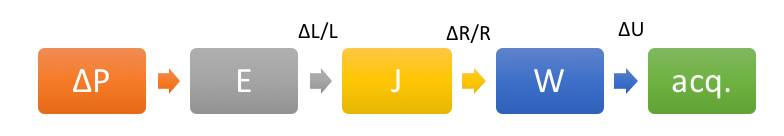
\includegraphics[scale=0.5]{image1.jpg} 
\end{center}

Losqu'on applique un effort F au capteur, un champ de contrainte apparait et donc des déformations apparaissent.Le corps d'épreuve est en effet soumis à allongement négatif suivant l'axe axial du fait de la compression(Loi de Hooke) d'une autre part nous avons un allongement suivant l'axe radial qui va agrandir le diamètre de la pièce (Coefficient de Poisson) Grâce à la loi de Pouillet , nous pourrons connaitre la variation de la résistance dans la jauge (un fil). En effet, lors des déformations de la pièce, la jauge se déforme également et donc modifie sa résistance (Annexe...). Nous pouvons négligé la résistivité ainsi que le volume. On introduit alors K qui est le facteur de jauge qui caractérise la variation de résistance en fonction de sa déformation axiale. Nous avons ici de très petites variations de résistance.
C'est pourquoi, la mesure ne peut s'effectuer directement avec un ohmètre. La première idée était d'utiliser un diviseur de tension (1 jauge / 1 resistance) mais afin d'annuler l'influence de la température sur la mesure nous utiliserons plutôt un pont de Wheatstone (2jauges / 2 résistances). Par ailleurs, on ne peut introduire deux jauges (pour corriger la tempèrature) que si celle si sont placées perpendiculairement (afin de conserver notre mesure de déformation, les deux jauges se déformant différemment avec un facteur \mu). L'utilisation d'un pont de Wheatstone, soit un circuit constitué de 4 résistances montées en pont et alimenté sous une tension de 5V ( Celle-ci ne peut être supérieur car même si la température dûe à l'effet Joule (Annexe...) n'est pas prise en compte dans nos mesures, elle pourrait décoler la jauge). A l'équilibre (pas de charge appliquée) la tension de sortie est nulle. Cependant, la variation d'une quelconque résistance dûe à la charge va faire apparaître une différence de potentiel. La tension de sortie est donc proportionnel aux variations relatives deltaR/R de chacunes des résistances. 

\section*{Liste du matériel}
\begin{itemize}
\item poids 
\item corps d'épreuve
\item huit jauges de déformations (type FCA-5-23)
\item un corps d'épreuve (diabolo en aluminium)
\item cinq charges experimentales de masse connue
\item un générateur de courant continu (5V)
\item Matériel d'acquisition (Ordinateur avec software dédié)   une Balance à levier
\end{itemize}	

\section*{Procédure}
\begin{center}
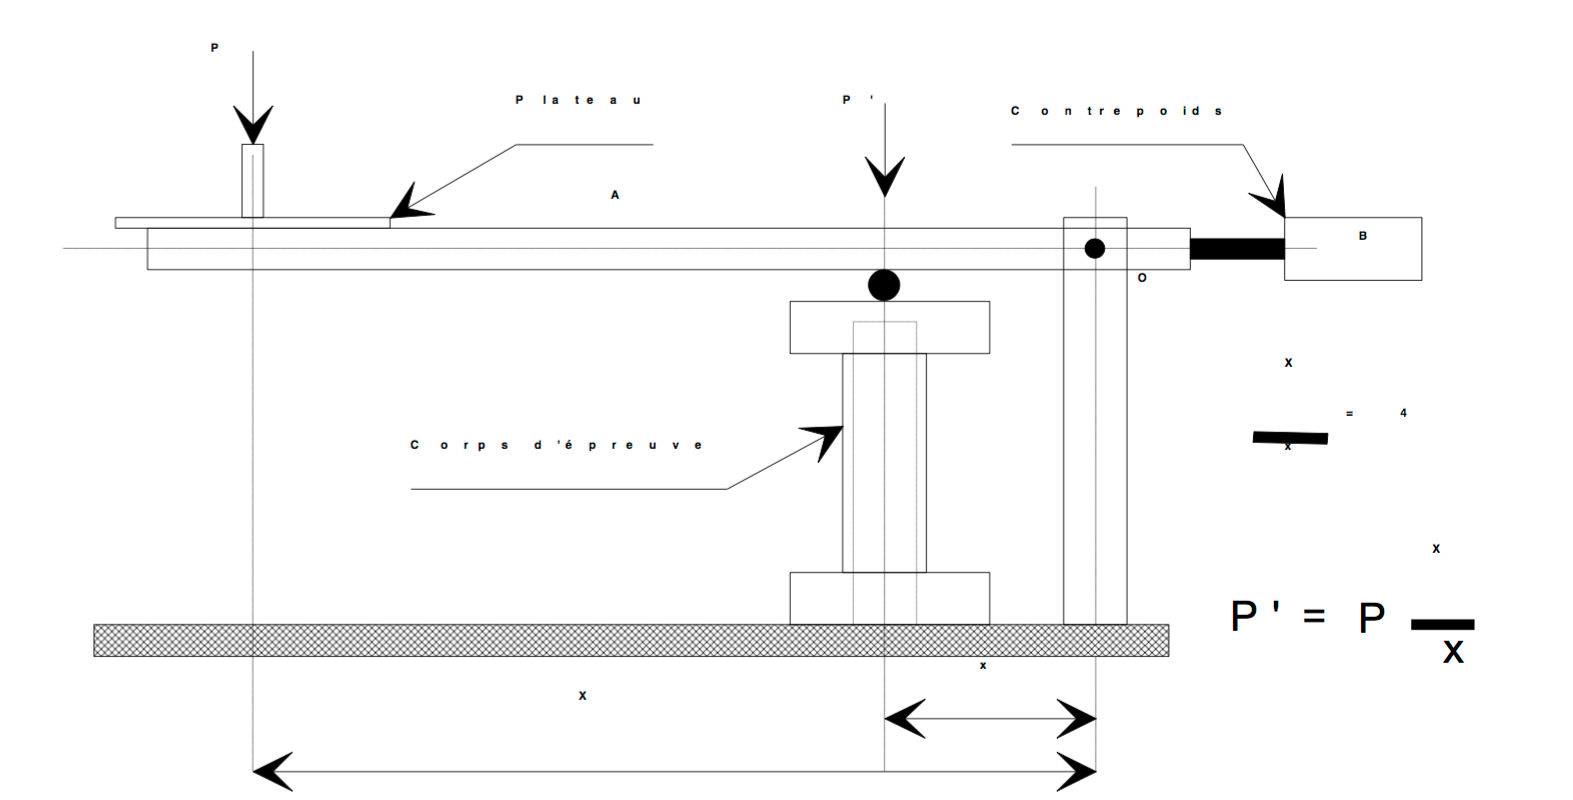
\includegraphics[scale=0.3]{Montage.jpg}
\end{center}
\begin{enumerate}
\item Tarrer du système pour la prise de mesure de la contrainte appliquée.									
\item Réquilibrer le pont de Wheatsone (Calibrage du 0V)
\item Center le corps d'épreuve sous la bille qui permet d'appliquer la charge.
\item Deposer la charge sur le plateau.
\item Relever la différence de potentiel  et la valeur de la masse affichée à l'écran
\item Repeter les opération 2 à 5 en augmentant la valeur de la charge par pas de 500g en veillant à ne pas déposer une charge supérieur à 5kg
\item Repeter la procédure pour des centrage de l'application de la contrainte différente
\end{enumerate} 


Il est important de rester délicat avec la matériel lors du changement de masse ou du changement de centrage d'application de la force, Sous peine de fausser les mesures suivantes. S'aider du sabot pour enlever la contrainte sur le diabolo lors du changement de masse.
\newpage
\section*{Mesures \& observations}
\subsection*{Graphique}
\begin{center}
~\\
Tension en fonction de la masse lorsque la contrainte est centrée~\\
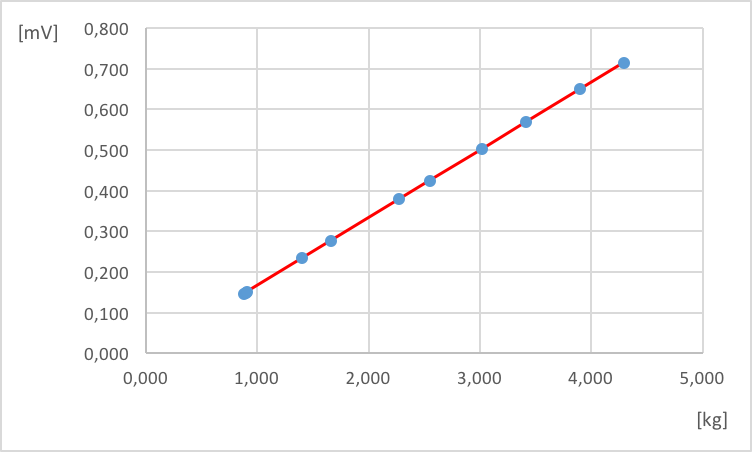
\includegraphics[scale=1]{Graphique1.png} ~\\~\\~\\~\\~\\~\\
Ecart relatif de la masse par rapport à la valeur de la masse lorsque la contrainte est centrée~\\
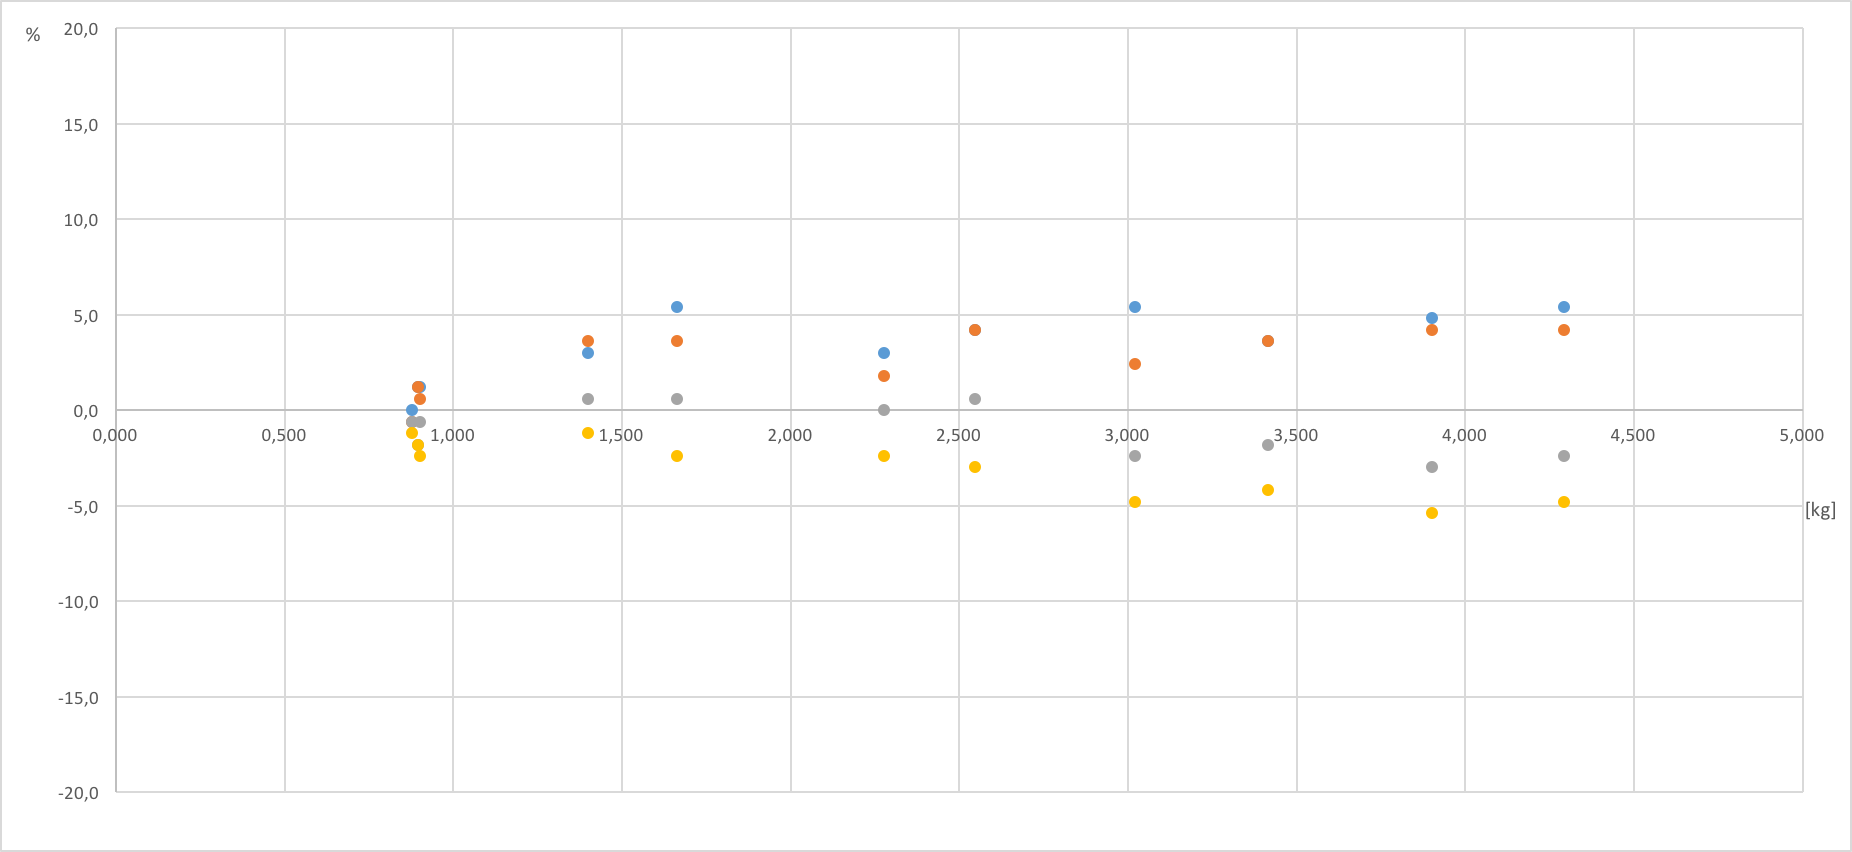
\includegraphics[scale=0.4]{Graphique2.png} ~\\
\end{center}
\newpage
\subsection*{Tableau de valeurs}
\begin{center}
~\\
Masse observée en fonction de la masse appliquée et de la position de la contrainte
\begin{tabular}{|c|c|c|c|c|c|c|}
\hline
\rowcolor[HTML]{036400} 
\cellcolor[HTML]{963400}{\color[HTML]{FFFFFF} N}        & \cellcolor[HTML]{963400}{\color[HTML]{FFFFFF} N} & {\color[HTML]{FFFFFF} Masse G2} & {\color[HTML]{FFFFFF} Masse G1} & {\color[HTML]{FFFFFF} Masse C}  & {\color[HTML]{FFFFFF} Masse D1} & {\color[HTML]{FFFFFF} Masse G2} \\ \hline
\rowcolor[HTML]{E7F7E7} 
\cellcolor[HTML]{FFECE2}{\color[HTML]{963400} {[}kg{]}} & \cellcolor[HTML]{FFECE2}{\color[HTML]{963400} }  & {\color[HTML]{036400} {[}kg{]}} & {\color[HTML]{036400} {[}kg{]}} & {\color[HTML]{036400} {[}kg{]}} & {\color[HTML]{036400} {[}kg{]}} & {\color[HTML]{036400} {[}kg{]}} \\ \hline
{\color[HTML]{963400} 0,584}                            & {\color[HTML]{963400} 4}                         & {\color[HTML]{036400} 0,500}    & {\color[HTML]{036400} 0,494}    & {\color[HTML]{036400} 0,512}    & {\color[HTML]{036400} 0,506}    & {\color[HTML]{036400} 0,512}    \\ \hline
{\color[HTML]{963400} 1,050}                            & {\color[HTML]{963400} 6}                         & {\color[HTML]{036400} 0,878}    & {\color[HTML]{036400} 0,884}    & {\color[HTML]{036400} 0,878}    & {\color[HTML]{036400} 0,884}    & {\color[HTML]{036400} 0,890}    \\ \hline
{\color[HTML]{963400} 1,056}                            & {\color[HTML]{963400} 5}                         & {\color[HTML]{036400} 0,884}    & {\color[HTML]{036400} 0,884}    & {\color[HTML]{036400} 0,896}    & {\color[HTML]{036400} 0,914}    & {\color[HTML]{036400} 0,914}    \\ \hline
{\color[HTML]{963400} 1,063}                            & {\color[HTML]{963400} 7}                         & {\color[HTML]{036400} 0,890}    & {\color[HTML]{036400} 0,896}    & {\color[HTML]{036400} 0,902}    & {\color[HTML]{036400} 0,908}    & {\color[HTML]{036400} 0,926}    \\ \hline
{\color[HTML]{963400} 1,640}                            & {\color[HTML]{963400} 4+5}                       & {\color[HTML]{036400} 1,370}    & {\color[HTML]{036400} 1,364}    & {\color[HTML]{036400} 1,400}    & {\color[HTML]{036400} 1,394}    & {\color[HTML]{036400} 1,412}    \\ \hline
{\color[HTML]{963400} 1,964}                            & {\color[HTML]{963400} 9}                         & {\color[HTML]{036400} 1,610}    & {\color[HTML]{036400} 1,628}    & {\color[HTML]{036400} 1,664}    & {\color[HTML]{036400} 1,658}    & {\color[HTML]{036400} 1,688}    \\ \hline
{\color[HTML]{963400} 2,690}                            & {\color[HTML]{963400} 4+5+6}                     & {\color[HTML]{036400} 2,246}    & {\color[HTML]{036400} 2,258}    & {\color[HTML]{036400} 2,276}    & {\color[HTML]{036400} 2,276}    & {\color[HTML]{036400} 2,300}    \\ \hline
{\color[HTML]{963400} 3,020}                            & {\color[HTML]{963400} 5+9}                       & {\color[HTML]{036400} 2,504}    & {\color[HTML]{036400} 2,504}    & {\color[HTML]{036400} 2,546}    & {\color[HTML]{036400} 2,540}    & {\color[HTML]{036400} 2,576}    \\ \hline
{\color[HTML]{963400} 3,604}                            & {\color[HTML]{963400} 5+9+4}                     & {\color[HTML]{036400} 2,966}    & {\color[HTML]{036400} 2,996}    & {\color[HTML]{036400} 3,020}    & {\color[HTML]{036400} 3,044}    & {\color[HTML]{036400} 3,068}    \\ \hline
{\color[HTML]{963400} 4,077}                            & {\color[HTML]{963400} 6+7+9}                     & {\color[HTML]{036400} 3,380}    & {\color[HTML]{036400} 3,380}    & {\color[HTML]{036400} 3,416}    & {\color[HTML]{036400} 3,434}    & {\color[HTML]{036400} 3,458}    \\ \hline
{\color[HTML]{963400} 4,661}                            & {\color[HTML]{963400} 6+7+9+4}                   & {\color[HTML]{036400} 3,854}    & {\color[HTML]{036400} 3,860}    & {\color[HTML]{036400} 3,902}    & {\color[HTML]{036400} 3,932}    & {\color[HTML]{036400} 3,956}    \\ \hline
{\color[HTML]{963400} 5,133}                            & {\color[HTML]{963400} 6+7+9+5}                   & {\color[HTML]{036400} 4,238}    & {\color[HTML]{036400} 4,250}    & {\color[HTML]{036400} 4,292}    & {\color[HTML]{036400} 4,316}    & {\color[HTML]{036400} 4,340}    \\ \hline
\end{tabular}
~\\~\\~\\~\\~\\
Différence de potentielle en fonction de la masse appliquée et de la position de la contrainte~\\
\begin{tabular}{|c|c|c|c|c|c|c|}
\hline
\rowcolor[HTML]{2A2AA1} 
\cellcolor[HTML]{963400}{\color[HTML]{FFFFFF} N}        & \cellcolor[HTML]{963400}{\color[HTML]{FFFFFF} N} & {\color[HTML]{FFFFFF} Tension G2} & {\color[HTML]{FFFFFF} Tension G1} & {\color[HTML]{FFFFFF} Tension C} & {\color[HTML]{FFFFFF} Tension D1} & {\color[HTML]{FFFFFF} Tension D2} \\ \hline
\rowcolor[HTML]{DDDDFF} 
\cellcolor[HTML]{FFECE2}{\color[HTML]{963400} {[}kg{]}} & \cellcolor[HTML]{FFECE2}{\color[HTML]{963400} }  & {\color[HTML]{2A2AA1} {[}mV{]}}   & {\color[HTML]{2A2AA1} {[}mV{]}}   & {\color[HTML]{2A2AA1} {[}mV{]}}  & {\color[HTML]{2A2AA1} {[}mV{]}}   & {\color[HTML]{2A2AA1} {[}mV{]}}   \\ \hline
{\color[HTML]{963400} 0,584}                            & {\color[HTML]{963400} 4}                         & {\color[HTML]{00009B} 0,083}      & {\color[HTML]{00009B} 0,082}      & {\color[HTML]{00009B} 0,085}     & {\color[HTML]{00009B} 0,084}      & {\color[HTML]{00009B} 0,085}      \\ \hline
{\color[HTML]{963400} 1,050}                            & {\color[HTML]{963400} 6}                         & {\color[HTML]{00009B} 0,146}      & {\color[HTML]{00009B} 0,147}      & {\color[HTML]{00009B} 0,146}     & {\color[HTML]{00009B} 0,147}      & {\color[HTML]{00009B} 0,148}      \\ \hline
{\color[HTML]{963400} 1,056}                            & {\color[HTML]{963400} 5}                         & {\color[HTML]{00009B} 0,147}      & {\color[HTML]{00009B} 0,147}      & {\color[HTML]{00009B} 0,149}     & {\color[HTML]{00009B} 0,152}      & {\color[HTML]{00009B} 0,151}      \\ \hline
{\color[HTML]{963400} 1,063}                            & {\color[HTML]{963400} 7}                         & {\color[HTML]{00009B} 0,148}      & {\color[HTML]{00009B} 0,149}      & {\color[HTML]{00009B} 0,150}     & {\color[HTML]{00009B} 0,151}      & {\color[HTML]{00009B} 0,154}      \\ \hline
{\color[HTML]{963400} 1,640}                            & {\color[HTML]{963400} 4+5}                       & {\color[HTML]{00009B} 0,228}      & {\color[HTML]{00009B} 0,227}      & {\color[HTML]{00009B} 0,233}     & {\color[HTML]{00009B} 0,232}      & {\color[HTML]{00009B} 0,235}      \\ \hline
{\color[HTML]{963400} 1,964}                            & {\color[HTML]{963400} 9}                         & {\color[HTML]{00009B} 0,268}      & {\color[HTML]{00009B} 0,271}      & {\color[HTML]{00009B} 0,277}     & {\color[HTML]{00009B} 0,276}      & {\color[HTML]{00009B} 0,281}      \\ \hline
{\color[HTML]{963400} 2,690}                            & {\color[HTML]{963400} 4+5+6}                     & {\color[HTML]{00009B} 0,374}      & {\color[HTML]{00009B} 0,376}      & {\color[HTML]{00009B} 0,379}     & {\color[HTML]{00009B} 0,379}      & {\color[HTML]{00009B} 0,383}      \\ \hline
{\color[HTML]{963400} 3,020}                            & {\color[HTML]{963400} 5+9}                       & {\color[HTML]{00009B} 0,416}      & {\color[HTML]{00009B} 0,417}      & {\color[HTML]{00009B} 0,424}     & {\color[HTML]{00009B} 0,423}      & {\color[HTML]{00009B} 0,429}      \\ \hline
{\color[HTML]{963400} 3,604}                            & {\color[HTML]{963400} 5+9+4}                     & {\color[HTML]{00009B} 0,494}      & {\color[HTML]{00009B} 0,499}      & {\color[HTML]{00009B} 0,502}     & {\color[HTML]{00009B} 0,507}      & {\color[HTML]{00009B} 0,511}      \\ \hline
{\color[HTML]{963400} 4,077}                            & {\color[HTML]{963400} 6+7+9}                     & {\color[HTML]{00009B} 0,563}      & {\color[HTML]{00009B} 0,563}      & {\color[HTML]{00009B} 0,569}     & {\color[HTML]{00009B} 0,572}      & {\color[HTML]{00009B} 0,576}      \\ \hline
{\color[HTML]{963400} 4,661}                            & {\color[HTML]{963400} 6+7+9+4}                   & {\color[HTML]{00009B} 0,642}      & {\color[HTML]{00009B} 0,643}      & {\color[HTML]{00009B} 0,650}     & {\color[HTML]{00009B} 0,654}      & {\color[HTML]{00009B} 0,659}      \\ \hline
{\color[HTML]{963400} 5,133}                            & {\color[HTML]{963400} 6+7+9+5}                   & {\color[HTML]{00009B} 0,706}      & {\color[HTML]{00009B} 0,708}      & {\color[HTML]{00009B} 0,715}     & {\color[HTML]{00009B} 0,718}      & {\color[HTML]{00009B} 0,723}      \\ \hline

\end{tabular}
\end{center}
\paragraph{Observation :} Nous avons constaté qu' au cours de l'expérimentation (après 45min) la valeur du zéro avait légèrement changée (+  0,001 mV pour la mesure de la tension). 
\section*{Interpretation}	
\section*{Conclusion}	
\section*{Annexe}	



\end{document}
